\section{算符及其性质}

\begin{quotation}
``伟大的数学家已经针对人类思想作出了甚至比文学家还更加不朽的贡献,因为它与语言无关。''\qquad 提奇马什
\end{quotation}

\begin{figure}[h]
\begin{center}
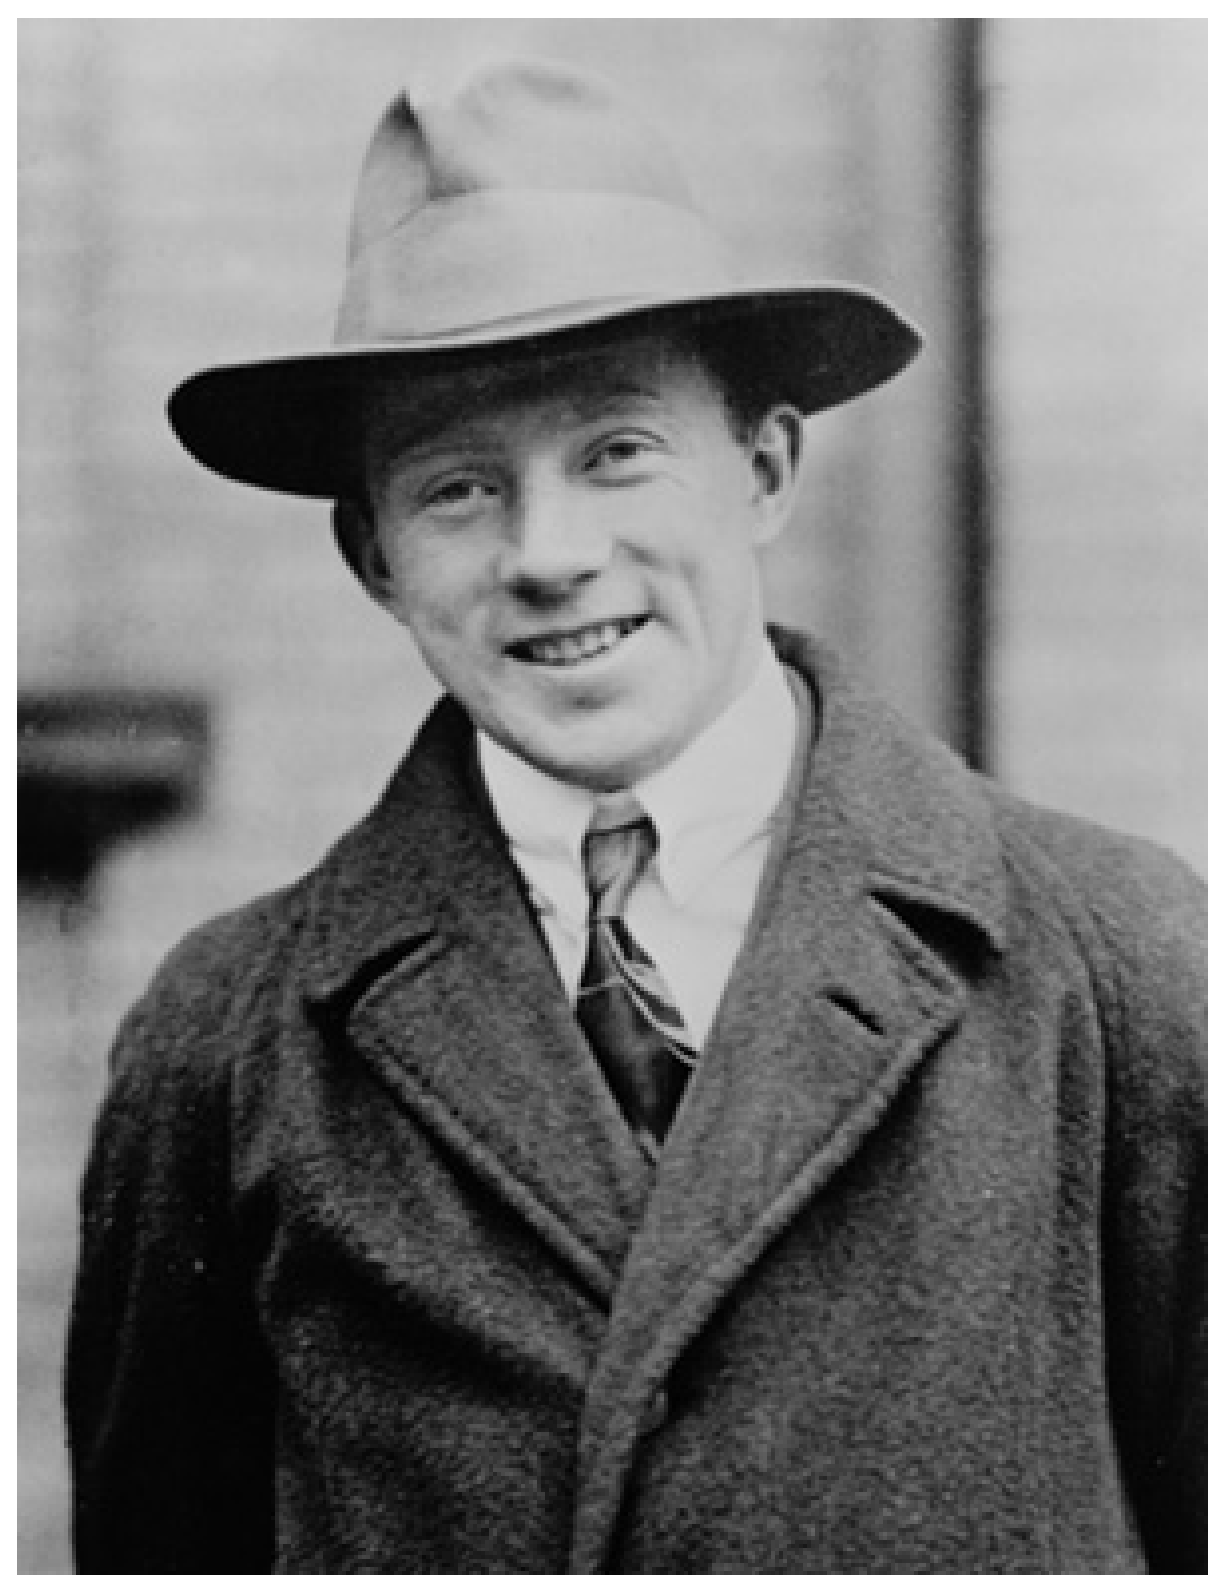
\includegraphics[clip,width=6cm]{Operators/heisenberg.ps}
\caption{海森堡}
\end{center}
\end{figure}

在量子力学中,用波函数描写微观粒子运动状态,波函数满足运动方程——薛定谔方程,而力学量则使用算符表示。
在已知波函数$\psi$情况下,力学量算符的平均值:$\left\langle {\hat F} \right\rangle  \equiv \overline F  = \int {\psi ^* \hat F\psi d\tau } $就对应力学量的测量值。

\subsection{算符的定义}

\subsubsection{算符的定义}

$u$,$v$是希尔波特空间中两个矢量(两个函数),若存在映射$\hat O:u
\to v$将一个矢量u映射到另一矢量v,则称映射$\hat
O$为算符\footnote{即算符作用于函数,使一个函数变为另外的函数。}。表示为:$\hat
Ou = v$

例如:$\frac{{du}}{{dx}} = v$中$\frac{{d}}{{dx}}$就是算符;

几个名称的定义:

\begin{itemize}
    \item \textbf{单位算符:}$\hat {\rm I}u = u$,$u$是任意函数;
    \item \textbf{零算符:}$\hat 0u = 0$,$u$是任意函数;
    \item 本征值方程:$\hat O u = \lambda u$,$\lambda$是本征值,$u$为属于$\lambda$的本征函数;
\end{itemize}

\subsubsection{算符的运算}

\begin{itemize}
    \item \textbf{算符相等:}如果:$\hat O_1 u = \hat O_2 u$,则:$\hat O_1 = \hat O_2$
    \item \textbf{算符之和:}如果:$\hat O u = \hat O_1 u + \hat O_2 u$,则:$\hat O = \hat O_1 + \hat O_2$
    \item \textbf{与参数相乘:}如果:$\hat O u = \lambda (\hat O_1 u)$,则:$\hat O = \lambda \hat O_1$
    \item \textbf{算符之积:}如果:$\hat O u = \hat O_1 (\hat O_2 u)$,则:$\hat O = \hat O_1 \hat O_2$
\end{itemize}
其中$u_1 ,u_2 $是任意函数,$\lambda$是复常数;

算符之和满足交换律、结合律\footnote{为了书写方便,以下我们也用不带尖帽的字母表示算符。}:$A + B = B + A,\left( {A + B} \right) + C = A + \left( {B + C} \right)$

算符之积不满足交换律:$AB \ne BA$,但满足结合律:$\left( {AB} \right)C = A\left( {BC} \right)$

\subsubsection{算符的对易}

\begin{itemize}
    \item \textbf{对易子:}$\left[ {A,B} \right] = AB - BA$

    \item \textbf{反对易子:}$\left\{ {A,B} \right\} = AB + BA$

    \item \textbf{对易式的性质:}

   $\begin{array}{l}
 \left[ {A,B} \right] =  - \left[ {B,A} \right] \\
 \left[ {A,\lambda } \right] = 0,\lambda  \in {\rm{C}} \\
 \left[ {A,B + C} \right] = \left[ {A,B} \right] + \left[ {A,C} \right] \\
 \left[ {A,BC} \right] = B\left[ {A,C} \right] + \left[ {A,B} \right]C \\
 \left[ {A,\left[ {B,C} \right]} \right] + \left[ {B,\left[ {C,A} \right]} \right] + \left[ {C,\left[ {A,B} \right]} \right] = 0 \\
 \end{array}$

    \item 对易式和反对易式的关系:

$\begin{array}{l}
 \left[ {AB,C} \right] = A\left\{ {B,C} \right\} - \left\{ {A,C} \right\}B \\
 \left[ {A,BC} \right] = \left\{ {A,B} \right\}C - B\left\{ {A,C} \right\} \\
 \end{array}$

\end{itemize}


\subsubsection{基础对易关系}

\textbf{练习1}: 计算对易关系 $\left[ {\hat x , \hat p_x } \right]$

$\hat x = x$,$\hat p_x  = \frac{\hbar }{i}\frac{d}{{dx}}$

$\begin{array}{l}
 \left( {\hat x \hat p_x  - \hat p_x \hat x} \right)\psi  = \left( {x\frac{\hbar }{i}\frac{d}{{dx}} - \frac{\hbar }{i}\frac{d}{{dx}}x} \right)\psi  = x\frac{\hbar }{i}\psi ' - \frac{\hbar }{i}\frac{d}{{dx}}x\psi  \\
  = x\frac{\hbar }{i}\psi ' - \frac{\hbar }{i}\left( {\psi  + x\psi '} \right) =  - \frac{\hbar }{i}\psi  = i\hbar \psi  \\
 \end{array}$

所以:$\left[ {\hat x,\hat p_x } \right] = i\hbar $

类似地:$\left[ {\hat y,\hat p_y } \right] = i\hbar $,$\left[ {\hat z,\hat p_z } \right] = i\hbar $;$\left[ {\hat x,\hat p_y } \right] = 0$,$\left[ {\hat p_x ,\hat p_y } \right] = 0$;......

一般写为:

\begin{equation}\label{fundamental commutation relations}
 \left[ {\hat x_i ,\hat p_j } \right] = i\hbar \delta _{ij}
\end{equation}

\index{Fundamental commutation relations: 基础对易关系}

这组对易关系也叫基础对易关系(Fundamental commutation relations),
狄拉克实际上就是以此作为基本条件建立起量子力学的\footnote{J. J.
Sakurai, \textbf{Modern Quantum Mechanics}, pp50},
当然在这里这组对易关系是作为推论计算出来的。存在多种建立量子力学的途径,
有薛定谔的波动力学, 海森堡的矩阵力学, 还有费曼的路径积分,
对于每种途径它们可以有不同的出发点, 当然最后得到的理论体系是一样的,
比如都有薛定谔方程$i \hbar \partial_t \psi = H \psi$,
它既可以在某些途径里作为基本假设直接提出来,
它也可以在其他途径里作为推论得到。


\subsubsection{波函数的内积}

$\left( {\psi ,\varphi } \right) = \int {\psi ^* \varphi d\tau } $

内积的性质:

\begin{itemize}
    \item $\left( {\psi ,\psi } \right) \ge 0$

    \item $\left( {\psi ,\varphi } \right)^*  = \left( {\varphi ,\psi } \right)$

    \item $\left( {\psi ,c_1 \varphi _1  + c_2 \varphi _2 } \right) = c_1 \left( {\psi ,\varphi _1 } \right) + c_2 \left( {\psi ,\varphi _2 } \right)$
   \end{itemize}




\subsection{算符的种类}

\subsubsection{线性算符}

定义:$O\left( {c_1 u_1  + c_2 u_2 } \right) = c_1 Ou_1  + c_2 Ou_2 $,其中:$u_1 ,u_2 $是任意函数,$c_1 ,c_2 $是任意复常数;

例:动量算符$\hat p = \frac{\hbar }{i}\nabla $是线性算符,平方算符不是线性算符$\left( {u_1  + u_2 } \right)^2  \ne u_1 ^2  + u_2 ^2 $;


\subsubsection{逆算符}

定义:设$Au = v$,存在算符$B$使$Bv = u$,则称:$A$,$B$互为逆算符:$B = A^{ - 1} ,A = B^{ - 1} $;

性质:

\begin{center}
$\begin{array}{l}
 A^{ - 1} A = AA^{ - 1}  = 1 \\
 \left( {A^{ - 1} } \right)^{ - 1}  = A \\
 \left( {\lambda A} \right)^{ - 1}  = \frac{1}{\lambda }A^{ - 1} ,\lambda  \ne 0 \\
 \left( {A_1 A_2 } \right)^{ - 1}  = A_2 ^{ - 1} A_1 ^{ - 1}  \\
 \end{array}$
\end{center}

\subsubsection{厄密共轭算符}


定义: 两个算符$A,B$满足:$\left( {\psi _1 ,A\psi _2 } \right) =
\left( {B\psi _1 ,\psi _2 } \right)$,即:$\int {\psi _1 ^* \left(
{A\psi _2 } \right)d\tau }  = \int {\psi _2 \left( {B\psi _1 }
\right)^* d\tau } $,则称:$A$,$B$互为厄密共厄算符:$B = A^ +  ,A =
B^ +  $


性质:

\begin{center}
$\begin{array}{l}
 \left( {A^ +  } \right)^ +   = A \\
 \left( {A_1  + A_2 } \right)^ +   = A_1 ^ +   + A_2 ^ +   \\
 \left( {\lambda A} \right)^ +   = \lambda ^* A^ +  ,\lambda  \in {\rm{C}} \\
 \left( {A_1 A_2 } \right)^ +   = A_2 ^ +  A_1 ^ +   \\
 \end{array}$
\end{center}

共轭算符可以定义为转置加复共轭:$O^ +   = \widetilde{O^* }$

\index{Hermitian adjoint: 厄米共轭}

\begin{center}
$\left( {\psi ,O\varphi } \right) = \left( {O^ +  \psi ,\varphi } \right) = \left( {O\varphi ,\psi } \right)^*  = \left( {O^* \varphi ^* ,\psi ^* } \right) = \left( {\widetilde{O^* }\psi ,\varphi } \right)$
\end{center}

转置算符定义\footnote{参考曾谨言《量子力学 卷I》第185页}:
$\left( {\psi ,\tilde O\varphi } \right) = \left( {\varphi ^* ,O\psi ^* } \right)$

觉得不好理解?实际上在采用了狄拉克记号后,这里的大部分定义和性质将看起来是自然而然的。

\subsubsection{幺正算符}

定义:$U^ +  U = 1$,$U^ +   = U^{ - 1} $

性质:$\left( {U\psi _1 ,U\psi _2 } \right) = \left( {\psi _1 ,U^ +  U\psi _2 } \right) = \left( {\psi _1 ,\psi _2 } \right)$

\subsubsection{厄密算符}

定义:如$A^ +   = A$,则称$A$为厄密算符;

\index{Hermitian operator: 厄米算符}

\begin{center}
$\left( {\psi _1 ,A\psi _2 } \right) = \left( {A\psi _1 ,\psi _2 } \right)$
\end{center}

性质1:厄密算符本征值是实数;

$A\psi  = a\psi $,$\left( {\psi ,A\psi } \right) = \left( {A\psi ,\psi } \right) = a\left( {\psi ,\psi } \right) = a^* \left( {\psi ,\psi } \right)$,所以:$a = a^* $

性质2:厄密算符相应于不同本征值的本征矢量必定正交;

$A\psi _m  = a_m \psi _m ,A\psi _n  = a_n \psi _n ,a_m  \ne a_n $,

$\left( {\psi _m ,A\psi _n } \right) = \left( {A\psi _m ,\psi _n } \right) = a_n \left( {\psi _m ,\psi _n } \right) = a_m ^* \left( {\psi _m ,\psi _n } \right) = a_m \left( {\psi _m ,\psi _n } \right)$,

$a_n \left( {\psi _m ,\psi _n } \right) - a_m \left( {\psi _m ,\psi _n } \right) = 0,a_n  - a_m  \ne 0$,所以:$\left( {\psi _m ,\psi _n } \right) = 0$

注:厄密算符相应于同一个本征值的各个简并本征矢量并不一定正交,但可以通过各个简并本征矢量的线性迭加构造出一组新的简并本征矢量,使得它们之间是相互正交的。

假设本征值$\lambda _n $是$f _n$重简并的,则有$f _n$个不同的本征矢量$\left\{ {\psi _{\lambda _n ,i} } \right\},i = 1,2,...,f_n $;

\begin{center}
$A\psi _{\lambda _n ,i}  = \lambda _n \psi _{\lambda _n ,i} ,i = 1,2,...,f_n $
\end{center}

线性迭加构造$f _n$个新本征矢,$\varphi _{\lambda _n ,j}  = \sum\limits_{i = 1}^{f_n } {c_{ji} \psi _{\lambda _n ,i} } ,j = 1,2,...,f_n $

新本征矢应是正交归一的:$\int {\varphi ^* _{\lambda _n ,j} \varphi _{\lambda _n ,l} d\tau }  = \delta _{j,l} ,j = 1,2,...,f_n ,l = 1,2,...,f_n $

由正交归一条件总可解出系数\footnote{归一条件:$f _n$个,正交条件:${\textstyle{1 \over 2}}f_n \left( {f_n  - 1} \right)$个,待定$c_{ji}$独立系数个数:${\textstyle{1 \over 2}}f_n \left( {f_n  + 1} \right)$}:$c_{ji} $。

性质3:

两厄密算符之和仍为厄密算符:$\left( {A + B} \right)^ +   = A^ +   + B^ +   = A + B$;

两厄密算符之积不一定是厄密算符,仅当两厄密算符对易时,其积是厄密算符;

\begin{center}
$\left( {AB} \right)^ +   = B^ +  A^ +   = BA = AB$
\end{center}


算符可用矩阵表示,对应也有:单位矩阵、逆矩阵、转置矩阵、厄密共轭、厄密等概念;

\subsubsection{练习}

\textbf{练习2}:如$A,B$是厄密算符,则${\textstyle{1 \over 2}}\left(
{AB + BA} \right),{\textstyle{1 \over {2i}}}\left( {AB - BA}
\right)$也是厄密算符;

${\textstyle{1 \over 2}}\left( {AB + BA} \right)^ +   = {\textstyle{1 \over 2}}\left( {B^ +  A^ +   + A^ +  B^ +  } \right) = {\textstyle{1 \over 2}}\left( {BA + AB} \right) = {\textstyle{1 \over 2}}\left( {AB + BA} \right)$

${\textstyle{1 \over {2i}}}\left( {AB - BA} \right) =  - {\textstyle{1 \over {2i}}}\left( {AB - BA} \right)^ +   =  - {\textstyle{1 \over {2i}}}\left( {BA - AB} \right) = {\textstyle{1 \over {2i}}}\left( {AB - BA} \right)$

\textbf{练习3}:证明动量算符$\hat p_x  = \frac{\hbar
}{i}\frac{\partial }{{\partial x}}$是厄密算符;

$\left( {\psi _1 ,\hat p_x \psi _2 } \right) = \frac{\hbar }{i}\int_{ - \infty }^\infty  {\psi _1 ^* \frac{d}{{dx}}} \psi _2 dx = \frac{\hbar }{i}\left[ {\psi _1 ^* \psi _2 } \right]_{ - \infty }^\infty   - \frac{\hbar }{i}\int_{ - \infty }^\infty  {\psi _2 d\psi _1 ^* } $

当$x \to  \pm \infty $,$\psi _1 ^* \psi _2  \to 0$

所以:

\begin{eqnarray*}
\left( {\psi _1 ,\hat p_x \psi _2 } \right) & = &  - \frac{\hbar
}{i}\int_{ - \infty }^\infty  {\psi _2 d\psi _1 ^* }  =  - \int_{ -
\infty }^\infty  {\psi _2 } \frac{\hbar }{i}\frac{{d\psi _1 ^*
}}{{dx}}dx \\
{} & = & \int_{ - \infty }^\infty  {\psi _2 \left( {\hat p_x
\psi _1 } \right)^* dx}  = \left( {\hat p_x \psi _1 ,\psi _2 }
\right)
\end{eqnarray*}


\subsection{力学量用算符表示}

在坐标表象下, 位置算符:$\hat r = r$;动量算符:$\hat p =
\frac{\hbar }{i}\nabla $。因此动能、势能和哈密顿量的算符也可用$\hat
r,\hat p$表示。
算符的定义可进一步推广到任意一个有经典对应的力学量或无经典对应的力学量,
如:自旋(spin)。

\subsubsection{有经典对应的力学量}

$F(r,p)$保持经典函数关系式不变,但将坐标和动量分别用算符代替;即:$\hat F = F(\hat r,\hat p) = F(r,{\textstyle{\hbar  \over i}}\nabla )$;

力学量平均值:

\begin{center}
$\begin{array}{l}
 \overline F  = \int {\psi ^* F\left( {r,{\textstyle{\hbar  \over i}}\nabla } \right)\psi d\tau }  = \left( {\psi ,\hat F \psi } \right) = \left\langle \psi  \right|\hat F\left| \psi  \right\rangle  \\
  = \left( {\sum\limits_m {c_m \phi _m } ,\sum\limits_n {\hat F c_n \phi _n } } \right) = \sum\limits_{m,n} {c^* _m c_n \lambda _n \left( {\phi _m ,\phi _n } \right)}  = \sum\limits_n {\left| {c_n } \right|} ^2 \lambda _n  \\
 \end{array}$
\end{center}

\textbf{练习4}:对轨道角动量: $\hat L = \hat r \times \hat p$, 证明$[L_x, L_y] = i\hbar L_z$; $[L_z, L^2]=0$.

证: (1)

\begin{equation*}
\hat L = \hat r \times \hat p = \left( {\begin{array}{*{20}c}
   i & j & k  \\
   x & y & z  \\
   {p_x } & {p_y } & {p_z }  \\
 \end{array} } \right)
\end{equation*}

因此:

\begin{eqnarray*}
% \nonumber to remove numbering (before each equation)
  L_x &=& yp_z - zp_y \\
  L_y &=& zp_x-xp_z \\
  L_z &=& xp_y - yp_x
\end{eqnarray*}

\begin{equation*}
[L_x, L_y] = [yp_z - zp_y, zp_x-xp_z]= [yp_z, zp_x] + [zp_y, xp_z]
\end{equation*}

这里需要反复使用: $[A, BC] = B[A,C]+ [A,B]C$这类恒等式. 比如:
$[yp_z, zp_x] =-i\hbar  y p_x$, $[zp_y, xp_z] = i\hbar x p_y$, 因此:

\begin{equation*}
[L_x, L_y] = i\hbar (x p_y - y p_x)=i\hbar L_z
\end{equation*}

这里我们还反复用到如下对易关系:

$[x, p_x]=i\hbar$, $[y, p_y]=i\hbar$, $[z, p_z]=i\hbar$;

$[x,y]=[y,z]=[z,x]=0$; $[p_x,p_y]=[p_y,p_z]=[p_z,p_x]=0$;

$[x, p_y]=[y,p_z]=[z,p_x]=...=0$.

类似地,我们还会得到:

\begin{equation*}
[L_y, L_z] =i\hbar L_x,  \quad [L_z, L_x] =i\hbar L_y. 
\end{equation*}

即:

$\hat L \times \hat L = \left( {\begin{array}{*{20}c}
   i & j & k  \\
   {\hat L_x } & {\hat L_y } & {\hat L_z }  \\
   {\hat L_x } & {\hat L_y } & {\hat L_z }  \\
\end{array}} \right) = \left( {\begin{array}{*{20}c}
   {\hat L_y \hat L_z  - \hat L_z \hat L_y }  \\
   {\hat L_z \hat L_x  - \hat L_x \hat L_z }  \\
   {\hat L_x \hat L_y  - \hat L_y \hat L_x }  \\
\end{array}} \right) = i \hbar \left( {\begin{array}{*{20}c}
   {\hat L_x }  \\
   {\hat L_y }  \\
   {\hat L_z }  \\
\end{array}} \right)$

(2) $L^2 = L_x^2 + L_y^2 + L_z^2$,

\begin{eqnarray*}
% \nonumber to remove numbering (before each equation)
  [L_z, L^2] &=& [L_z, L_x^2]+[L_z,
L_y^2] \\
  {} &=& L_x[L_z,L_x]+[L_z,L_x]L_x+L_y[L_z, L_y]+[L_z,L_y]L_y \\
  {} &=& i\hbar L_xL_y + i\hbar L_y L_x -i\hbar L_y L_x - i\hbar L_x
  L_y \\
  {} &=& 0
\end{eqnarray*}

类似可得:

\begin{equation*}
[L_x, L^2] = 0 , \quad [L_y, L^2] = 0  
\end{equation*}


此外,还可证明:$\left[ {\hat L_\alpha  ,x_\beta  } \right] = \varepsilon _{\alpha \beta \gamma } i\hbar x_\gamma  $;
$\left[ {\hat L_\alpha  ,\hat p_\beta  } \right] = \varepsilon _{\alpha \beta \gamma } i\hbar \hat p_\gamma  $

这里$\varepsilon _{\alpha \beta \gamma } $为反对称三维张量,
称为列维-斯维塔(Levi-Civita)记号;( $\varepsilon _{\alpha \beta
\gamma }  = 1$,$\alpha ,\beta ,\gamma $是$x,y,z$的偶置换;
$\varepsilon _{\alpha \beta \gamma }  = - 1$,$\alpha ,\beta ,\gamma
$是$x,y,z$的奇置换; $\varepsilon _{\alpha \beta \gamma }  =
0$,有两个或三个指标相同;)

\subsubsection{算符的函数}


算符$\hat A$的函数$F(\hat A)$可以表示为算符$\hat A$的幂级数的形式:$F(\hat A) = \sum\limits_{n = 0}^\infty  {\frac{{F^{(n)} \left( 0 \right)}}{{n!}}\hat A^n } $,其中导数定义同函数$F(x)$的导数定义:$F(x) = \sum\limits_{n = 0}^\infty  {\frac{{F^{(n)} \left( 0 \right)}}{{n!}}x^n } $


\textbf{练习5}:平移算符

\index{Translation operator: 平移算符}

首先证明:$\exp \left[ {a{\textstyle{d \over {dx}}}} \right]\psi (x) = \psi (x + a)$

$\exp \left[ {a{\textstyle{d \over {dx}}}} \right]\psi (x) = \sum\limits_{n = 0}^\infty  {\frac{{a^n {\textstyle{{d^n } \over {dx^n }}}}}{{n!}}} \psi (x) = \sum\limits_{n = 0}^\infty  {\frac{{a^n \psi ^{(n)} (x)}}{{n!}}} $

$\psi (x + a) = \sum\limits_{n = 0}^\infty  {\frac{{a^n \psi ^{(n)} (x)}}{{n!}}} $

可以定义平移算符为:

\begin{equation}
\hat T(a) = \exp \left[ {a\frac{d}{{dx}}} \right] = \exp \left[ {a\frac{i}{\hbar }\frac{\hbar }{i}\frac{d}{{dx}}} \right] = \exp \left[ {\frac{{i\hat pa}}{\hbar }} \right]
\end{equation}

可以证明平移算符是幺正算符:$\hat T^ +  \hat T = \hat 1$

\subsection{练习:算符的函数Glauber公式}

\index{Glauber formula: Glauber公式}

算符的指数函数可定义为:$\exp \left[ {\hat A} \right] = 1 + \hat A + \frac{{\hat A^2 }}{{2!}} + ... + \frac{{\hat A^n }}{{n!}} + ...$

(1)证明:$\frac{d}{{dt}}\exp \left[ {t\hat A} \right] = \hat A\exp \left[ {t\hat A} \right] = \exp \left[ {t\hat A} \right]\hat A$,$t \in {\rm{C}}$

(2)$\hat A, \hat B$是两个算符,把$\exp \left[ {\hat A} \right]$按幂级数直接展开,比较同次幂系数,
验证等式:$e^{\hat A} \hat Be^{ - \hat A}  = \hat B + \left[ {\hat A,\hat B} \right] + \frac{1}{{2!}}\left[ {\hat A,\left[ {\hat A,\hat B} \right]} \right] + ... + \frac{1}{{n!}}\left[ {\hat A,\left[ {\hat A,...\left[ {\hat A,\hat B} \right]} \right]} \right] + ...$成立;

(3)定义算符的函数:$\hat F(t) = e^{t\hat A} \hat Be^{ - t\hat A} $,$t \in {\rm{C}}$

把算符的函数$\hat F(t)$按$t$的幂级数展开:$\hat F(t) = \sum\limits_{n = 0}^\infty  {\frac{{t^n \hat F^{(n)} \left( 0 \right)}}{{n!}}} $;$\hat F^n (0) = \left. {\frac{{d^n }}{{dt^n }}\hat F(t)} \right|_{t = 0} $

证明:$\hat F(t) = \sum\limits_{n = 0}^\infty  {\frac{{t^n }}{{n!}}\hat F_n } $,这里:$\hat F_0  = \hat B,\hat F_1  = \left[ {\hat A,\hat B} \right],\hat F_2  = \left[ {\hat A,\left[ {\hat A,\hat B} \right]} \right],...$

如令$t = 1$,则得到$e^{\hat A} \hat Be^{ - \hat A}  = \hat B + \left[ {\hat A,\hat B} \right] + \frac{1}{{2!}}\left[ {\hat A,\left[ {\hat A,\hat B} \right]} \right] + ... + \frac{1}{{n!}}\left[ {\hat A,\left[ {\hat A,...\left[ {\hat A,\hat B} \right]} \right]} \right] + ...$\\



(4)如果:$\left[ {\hat A,\left[ {\hat A,\hat B} \right]} \right] = \left[ {\hat B,\left[ {\hat A,\hat B} \right]} \right] = 0$,证明Glauber公式:$e^{\hat A} e^{\hat B}  = e^{\hat A + \hat B} e^{{\textstyle{1 \over 2}}\left[ {\hat A,\hat B} \right]} $;


(4.1)把等式左边$e^{\hat A} ,e^{\hat B} $按幂级数直接展开到二次方项,忽略更高次方项;
把等式右面:$e^{\hat A + \hat B} e^{{\textstyle{1 \over 2}}\left[ {\hat A,\hat B} \right]}  = e^{\hat A + \hat B + {\textstyle{1 \over 2}}\left[ {\hat A,\hat B} \right]} $也按幂级数直接展开,忽略更高次方项;
验证等式$e^{\hat A} e^{\hat B}  = e^{\hat A + \hat B} e^{{\textstyle{1 \over 2}}\left[ {\hat A,\hat B} \right]} $成立;


(4.2)令:$\hat C = \left[ {\hat A,\hat B} \right]$,$\left[ {\hat A,\hat C} \right] = \left[ {\hat B,\hat C} \right] = 0$;反复利用:$\left[ {A,BC} \right] = B\left[ {A,C} \right] + \left[ {A,B} \right]C$,
证明:$\left[ {\hat A,\hat B^n } \right] = n\hat C\hat B^{n - 1} $;

并在此基础上证明,$\left[ {\hat A,e^{t\hat B} } \right] = t\hat Ce^{t\hat B} $(提示:把等式左边指数函数按幂级数展开)

(4.3)定义函数:$G(t) = e^{t\hat A} e^{t\hat B} $,$H(t) = e^{t(\hat A + \hat B)} e^{{\textstyle{1 \over 2}}t^2 \hat C} $

证明:初始条件:$G_{t = 0}  = H_{t = 0} $,
微分关系:$\frac{d}{d}G(t) = G(t)\left( {\hat A + \hat B + t\hat C} \right)$,$\frac{d}{{dt}}H(t) = H(t)\left( {\hat A + \hat B + t\hat C} \right)$

证明:$G(t) = H(t)$,当$t = 1$时,得到等式:$e^{\hat A} e^{\hat B}  = e^{\hat A + \hat B} e^{{\textstyle{1 \over 2}}\left[ {\hat A,\hat B} \right]}  = e^{\hat A + \hat B + {\textstyle{1 \over 2}}\left[ {\hat A,\hat B} \right]} $

解:为简单计,我们用大写字母,如$A$,
$B$等表示算符,用小写字母$t$表示参数。

(1)

$\begin{array}{l}
 \frac{d}{{dt}}e^{tA}  = \sum\limits_{n = 0}^\infty  {\frac{d}{{dt}}\left( {\frac{{t^n A^n }}{{n!}}} \right)}  = \sum\limits_{n = 1}^\infty  {A\frac{{t^{n - 1} A^{n - 1} }}{{\left( {n - 1} \right)!}}}  = \sum\limits_{n = 1}^\infty  {\frac{{t^{n - 1} A^{n - 1} A}}{{\left( {n - 1} \right)!}}}  \\
  = Ae^{tA}  = e^{tA} A \\
 \end{array}$

 (2)

 $\begin{array}{l}
 e^A  = 1 + A + \frac{1}{{2!}}A^2  + ... + \frac{1}{{n!}}A^n  + ... \\
 e^{ - A}  = 1 - A + \frac{1}{{2!}}A^2  + ... + \frac{{\left( { - 1} \right)^n }}{{n!}}A^n  + ... \\
 \end{array}$


代入$e^A Be^{ - A} $得到:

$\begin{array}{l}
 e^A Be^{ - A}  \\
  = \left( {1 + A + \frac{1}{{2!}}A^2  + ... + \frac{1}{{n!}}A^n   ...} \right)B\left( {1 - A + \frac{1}{{2!}}A^2  + ... + \frac{{\left( { - 1} \right)^n }}{{n!}}A^n   ...} \right) \\
  = \left( {B + AB + \frac{1}{{2!}}A^2 B + ...\frac{1}{{n!}}A^n B  ...} \right)\left( {1 - A + \frac{1}{{2!}}A^2  + ... + \frac{{\left( { - 1} \right)^n }}{{n!}}A^n   ...} \right) \\
  = ... = B + \left[ {A,B} \right] + \frac{1}{{2!}}\left[ {A,\left[ {A,B} \right]} \right] + ... + \frac{1}{{n!}}\left[ {A,\left[ {A,...\left[ {A,B} \right]} \right]} \right]  ... \\
 \end{array}$

(3)

算符的函数$F\left( t \right) = e^{tA} Be^{ - tA} $,
把它按参数$t$展开为级数的形式:
$F\left( t \right) = \sum\limits_{n = 0}^\infty  {\frac{{t^n F^{(n)} \left( {t = 0} \right)}}{{n!}}} $;
这里$F^{(n)} \left( {t = 0} \right)$表示$t=0$时的$n$次导数。

一次导数:$\frac{{dF\left( t \right)}}{{dt}} = e^{tA} ABe^{ - tA}  + e^{tA} B\left( { - A} \right)e^{ - tA}  = e^{tA} \left[ {A,B} \right]e^{ - tA} $

二次导数:$\frac{{d^2 F\left( t \right)}}{{dt^2 }} = e^{tA} \left[ {A,\left[ {A,B} \right]} \right]e^{ - tA} $

一直计算到$n$次导数:$\frac{{d^n F\left( t \right)}}{{dt^n }} = e^{tA} \left[ {A,\left[ {A,...\left[ {A,B} \right]} \right]} \right]e^{ - tA} $,
这里包含有$n$次对易运算.

所以:

$\left\{ \begin{array}{l}
 \left. {\frac{{dF}}{{dt}}} \right|_{t = 0}  = \left[ {A,B} \right] \\
 \left. {\frac{{d^2 F}}{{dt^2 }}} \right|_{t = 0}  = \left[ {A,\left[ {A,B} \right]} \right] \\
 ... \\
 \left. {\frac{{d^n F}}{{dt^n }}} \right|_{t = 0}  = \left[ {A,\left[ {A,...\left[ {A,B} \right]} \right]} \right] \\
 \end{array} \right.$

根据定义:$F\left( t \right) = \sum\limits_{n = 0}^\infty  {\frac{{t^n }}{{n!}}F_n } $

求出:$F_0  = B,F_1  = \left[ {A,B} \right],F_2  = \left[ {A,\left[ {A,B} \right]} \right],...$

令$t=1$,

$F\left( 1 \right) = e^A Be^{ - A}  = B + \left[ {A,B} \right] + \frac{1}{{2!}}\left[ {A,\left[ {A,B} \right]} \right] + ... + \frac{1}{{n!}}\left[ {A,\left[ {A,...\left[ {A,B} \right]} \right]} \right] + ...$

(4.1)

$\begin{array}{l}
 e^A  = 1 + A + \frac{{A^2 }}{2} + O\left( 3 \right) \\
 e^B  = 1 + B + \frac{{B^2 }}{2} + O\left( 3 \right) \\
 \end{array}$


$\begin{array}{l}
 e^A e^B  = 1 + A + B + \frac{{A^2 }}{2} + \frac{{B^2 }}{2} + AB + O\left( 3 \right) \\
 e^{A + B}  = 1 + A + B + \frac{1}{2}\left( {A^2  + AB + BA + B^2 } \right) + O\left( 3 \right) \\
 e^{\frac{1}{2}\left[ {A,B} \right]}  = 1 + \frac{1}{2}\left[ {A,B} \right] + O\left( 4 \right) \\
 \end{array}$


容易验证在展开到二介小量条件下:$e^A e^B  = e^{A + B} e^{\frac{1}{2}\left[ {A,B} \right]} $

(4.2)

利用$\left[ {A,\left[ {A,B} \right]} \right] = 0$,$e^A Be^{ - A}  = ... = B + \left[ {A,B} \right]$



因此:$e^A B = Be^A  + \left[ {A,B} \right]e^A $


利用:$\left[ {A,B} \right] = C$ , $e^A B = Be^A  + Ce^A $



所以:$\left[ {e^A ,B} \right] = Ce^A $


类似地,利用 $\left[ {B,\left[ {A,B} \right]} \right] = 0$,
$e^{tB} Ae^{ - tB}  = ... = A + \left[ {B,A} \right]t$


所以:$\left[ {A,e^{tB} } \right] = tCe^{tB} $



利用$B$与$C$对易,

$\begin{array}{l}
 \left[ {A,B^n } \right] = B\left[ {A,B^{n - 1} } \right] + \left[ {A,B} \right]B^{n - 1}  \\
  = B\left\{ {B\left[ {A,B^{n - 2} } \right] + \left[ {A,B} \right]B^{n - 2} } \right\} + \left[ {A,B} \right]B^{n - 1}  \\
  = ... = nCB^{n - 1}  \\
 \end{array}$


直接计算,可得到:$\left[ {A,e^{tB} } \right] = \left[ {A,\sum\limits_{n = 0}^\infty  {\frac{{t^n B^n }}{{n!}}} } \right] = ... = tCe^{tB} $


(4.3)

初条件:$G_{t = 0}  = H_{t = 0}  = 1$

$G' = \frac{{dG(t)}}{{dt}} = e^{tA} Ae^{tB}  + e^{tA} Be^{tB} $


利用:$\left[ {A,e^{tB} } \right] = tCe^{tB} $,
$Ae^{tB}  = e^{tB} A + tCe^{tB} $


代入$G'$ 化简得到:$G' = e^{tA} e^{tB} \left( {A + B + tC} \right)$


类似地:

$\begin{array}{l}
 H' = \frac{{dH}}{{dt}} = e^{t\left( {A + B} \right)} \left( {A + B} \right)e^{\frac{{t^2 }}{2}C}  + e^{t\left( {A + B} \right)} tCe^{\frac{{t^2 }}{2}C}  \\
  = e^{t\left( {A + B} \right)} e^{\frac{{t^2 }}{2}C} \left( {A + B} \right) + e^{t\left( {A + B} \right)} e^{\frac{{t^2 }}{2}C} tC \\
  = H\left( t \right)\left( {A + B + tC} \right) \\
 \end{array}$


所以: $\frac{{G'}}{G} = \frac{{H'}}{H} = A + B + tC$



积分:

$\begin{array}{l}
 \int_0^t {\frac{{G'}}{G}dt}  = \int_0^t {\left( {\ln G} \right)^\prime  dt}  = \left[ {\ln G} \right]_0^t  = \ln G\left( t \right) - \ln G\left( 0 \right) \\
  = \int_0^t {\left( {A + B + tC} \right)dt}  = \left( {A + B} \right)t + \frac{{t^2 }}{2}C \\
 \end{array}$


所以:$G\left( t \right) = H\left( t \right) = e^{tA} e^{tB}  = e^{t\left( {A + B} \right)} e^{\frac{{t^2 }}{2}C}  = e^{\left( {A + B} \right)t + \frac{{t^2 }}{2}C} $



$t=1$代入上式:$e^A e^B  = e^{A + B} e^{\frac{1}{2}\left[ {A,B} \right]}  = e^{A + B + \frac{1}{2}\left[ {A,B} \right]} $


\subsection{正则变换}

利用

\begin{equation}\label{exp exp expansion}
 e^A Be^{ - A}  = B + [A,B] + \frac{1}{{2!}}[A,[A,B]] + ... +
\frac{1}{{n!}}[A,[A,...[A,B]]] + ...
\end{equation}

\index{Canonical transformation: 正则变换}

可得到近似求解哈密顿本征值的方法。1953年,中岛(S.
Nakajima)利用正则变换(Canonical
transformations)由``电子-声子哈密顿量''推出了Frohlich有效哈密顿量\footnote{参考:
李正中, 《固体理论》第二版, 第五章.

原始文献: S. Nakajima, Adv Phys, 1953, 4: 463}。

考虑哈密顿: $H = H_0 + H_1$,
哈密顿由主要部分$H_0$和微扰部分$H_1$组成, 我们关心的本征值问题是: $H
\psi = E \psi$。

现在作正则变换: $\psi \to e^{-S} \psi $, 则有: $ e^{-S} H e^S
e^{-S}\psi = E e^{-S} \psi$。

令$H_S = e^{-S} H e^{S}$, $\psi' = e^{-S} \psi$, $H_S \psi' = E
\psi'$, 即正则变换后的能量本征值与变换前的相同。

根据式\ref{exp exp expansion}, 得到:

\begin{equation*}
 \begin{array}{l}
 H_S  = H + [H,S] + \frac{1}{2}[[H,S],S] + ... \\
  = H_0  + \left( {H_1  + [H_0 ,S]} \right) + \frac{1}{2}\left[ {\left( {H_1  + [H_0 ,S]} \right),S} \right] + \frac{1}{2}[H_1 ,S] + ... \\
 \end{array}
\end{equation*}


选择变换$S$使满足: $H_1 + [H_0, S] = 0$, 则得到有效哈密顿量:

\begin{equation*}
 H_{eff} \approx H_0 + \frac{1}{2}[H_1 ,S]
\end{equation*}


\textbf{思考}:现在把$H_1$改写成$\lambda H_1$, $\lambda$表示小量,
重复以上推导, 看看得到的有效哈密顿是关于几阶小量的\footnote{参考:
``Time-dependent Frohlich transformation approach for two-atom
entanglement generated by successive passage through a cavity'',
\url{http://cn.arxiv.org/abs/quant-ph/0610102}}。

\subsection*{阅读与思考}

\begin{itemize}
    \item 复习:线性代数,如:

周士勋《量子力学教程》 附录

F.W. 拜仑, R.W. 富勒 《物理学中的数学方法 第一卷》

   \end{itemize}
